\begin{IEEEbiography}[{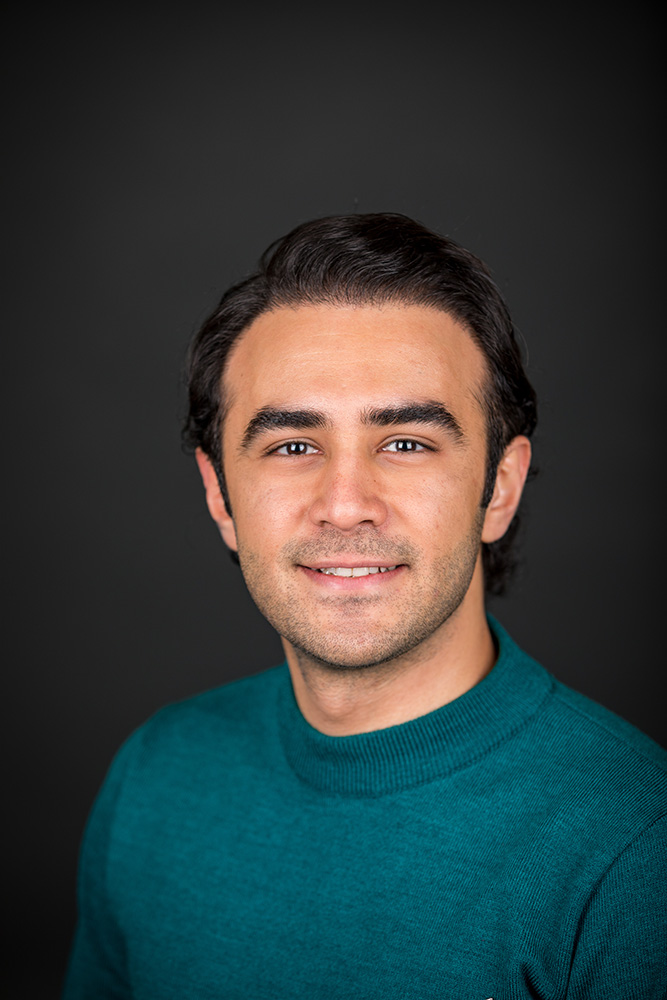
\includegraphics[width=1in,height=1.25in,clip,keepaspectratio]{Headshot.JPG}}]{Arshia Ilaty}
received the B.S. degree in computer engineering from the University of Tabriz, Iran, NV, USA, in 2021, and the M.S. degree in computer science and engineering from the University of Nevada, Reno, NV, USA, in 2023. He is currently pursuing the Ph.D. degree in computational science through a joint program at San Diego State University and the University of California, Irvine, CA, USA. His major field of study is applied machine learning and scientific computing, with a focus on healthcare and human-centered AI systems.

He has research experience spanning academia and industry. He has served as a Graduate Research Assistant at San Diego State University and the University of California, Irvine, where he develops agentic and multimodal AI systems for clinical trial optimization, pain assessment, and privacy-preserving synthetic data generation. Previously, he worked as a Software Engineer at World Mobile Inc., where he designed scalable cloud and blockchain-based systems, and as a Software Engineering Intern at Tesla, contributing to data-driven operational tooling and optimization. His research interests include multimodal machine learning, reinforcement learning, synthetic data generation, explainable AI, and high-performance computing for scientific and biomedical applications.

Mr. Ilaty is a member of the Association for Computing Machinery (ACM) and the Society for Industrial and Applied Mathematics (SIAM). He is the recipient of the Presidential Graduate Research Fellowship (UCI/SDSU), the Outstanding International Graduate Student Scholarship, and the WAAIME Scholarship. He has contributed to open-source scientific computing projects, including the libCEED and MOLE library, and has presented his work at academic conferences in applied AI.
\end{IEEEbiography}

\begin{IEEEbiography}[{\includegraphics[width=1in,height=1.25in,clip,keepaspectratio]{Shirazi.png}}]{Hossein Shirazi}
received the Ph.D. degree in electrical and computer engineering from Colorado State University, Fort Collins, CO, USA, in 2020. He is currently an Assistant Professor of Management Information Systems with the Fowler College of Business, San Diego State University, San Diego, CA, USA, where he directs the Smart Secure Systems (3S) Lab. 

His research interests lie at the intersection of cybersecurity and artificial intelligence, with specific focuses on Internet of Things (IoT) security, critical infrastructure protection, malware analysis, and adversarial machine learning. He has authored numerous publications in top-tier journals and conferences regarding the application of machine learning to enhance network security and resiliency.
\end{IEEEbiography}

\begin{IEEEbiography}[{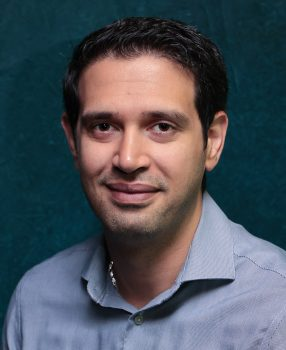
\includegraphics[width=1in,height=1.25in,clip,keepaspectratio]{Rahmani.jpg}}]{Amir M. Rahmani}
received the Ph.D. degree in computer systems from the University of Turku, Finland, in 2012, and the M.B.A. degree. He is currently a Professor with the School of Nursing and the Department of Computer Science, University of California, Irvine (UCI), Irvine, CA, USA. He is also the Founder and Director of the Health SciTech Group at UCI.

His interdisciplinary research bridges computer science and healthcare, focusing on e-health, m-health, wearable Internet of Things (IoT), bio-signal processing, and edge computing. He has led various projects on remote patient monitoring, pain assessment, and personalized healthcare systems. Dr. Rahmani has published extensively in the fields of embedded systems and healthcare IoT and serves on the editorial boards of several international journals.
\end{IEEEbiography}

\begin{IEEEbiography}[{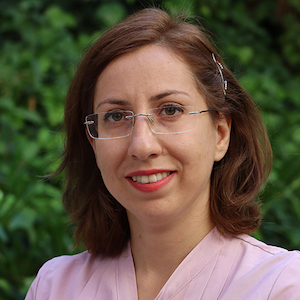
\includegraphics[width=1in,height=1.25in,clip,keepaspectratio]{homayouni.jpeg}}]{Hajar Homayouni}
received the Ph.D. degree in computer science from Colorado State University, Fort Collins, CO, USA, in 2020. She is currently an Assistant Professor with the Department of Computer Science, San Diego State University, San Diego, CA, USA, where she leads the Data Science Lab.

Her research interests include data quality, trustworthy artificial intelligence, big data management, and database systems. Her work focuses on developing methodologies to detect and repair data defects to ensure the reliability, fairness, and robustness of machine learning models. She is a member of the ACM and actively publishes in venues related to data engineering and applied AI.

\end{IEEEbiography}
